\section{Software}

\begin{frame}{Software}
	\begin{block}{Google Cast}
		Chromecast es un dispositivo que actúa como receptor y es compatible con el protocolo propietario Google Cast.
		Para iniciar la reproducción de un contenido pulsamos el botón de \textit{cast}.
	\end{block}

	\begin{figure}[h]
		\centering
		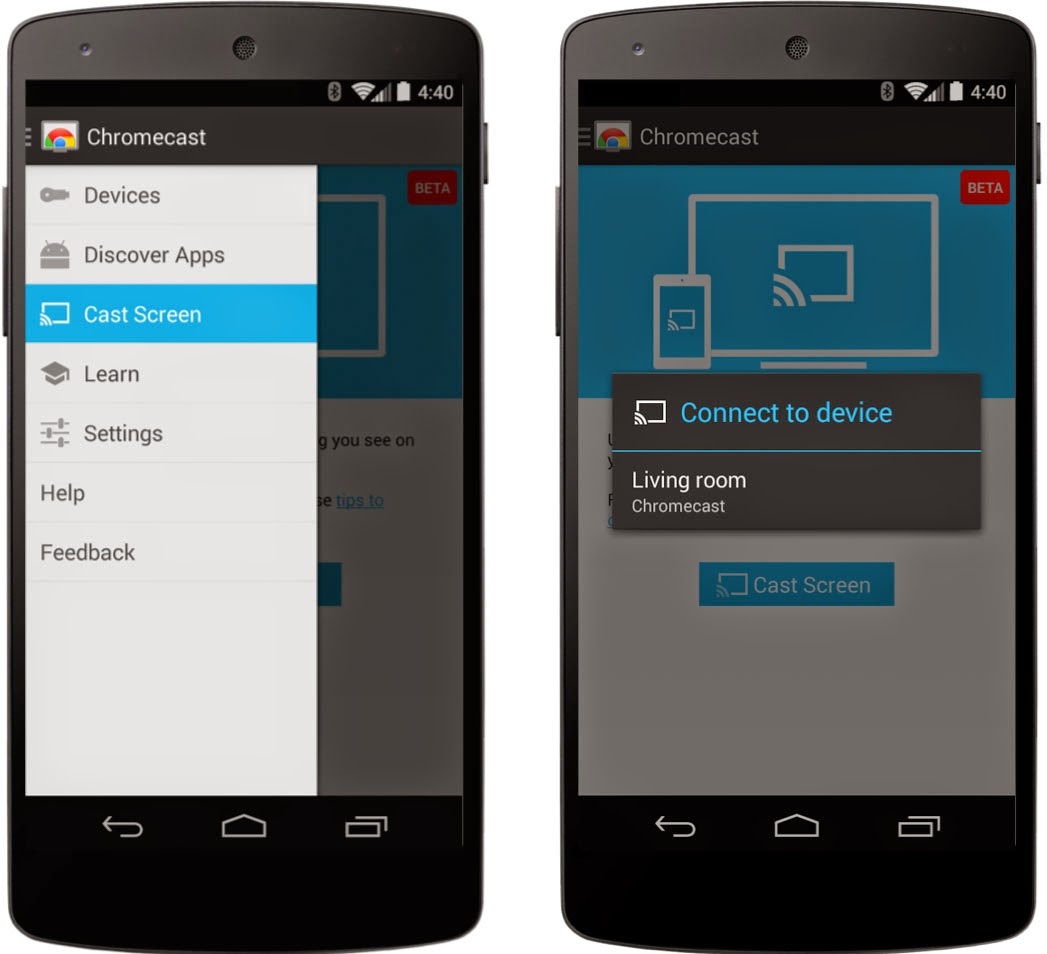
\includegraphics[width=0.5\textwidth]{./Imagenes/chromecast-mirroring.jpg}
	\end{figure}
\end{frame}



\subsection{Modos de funcionamiento}

\begin{frame}{Funcionamiento}
	\begin{block}{Primer modo}
		Usar el dispositivo emisor para controlar la reproducción. El receptor (p. ej.: Chromecast) se encarga de descargarlo del servidor, liberando al emisor de esta tarea.
		Esto permite al emisor ahorrar batería. Puede estar bloqueado o ejecutando simultáneamente otra aplicación mientras la reproducción tiene lugar.
	\end{block}

	\begin{figure}[h]
		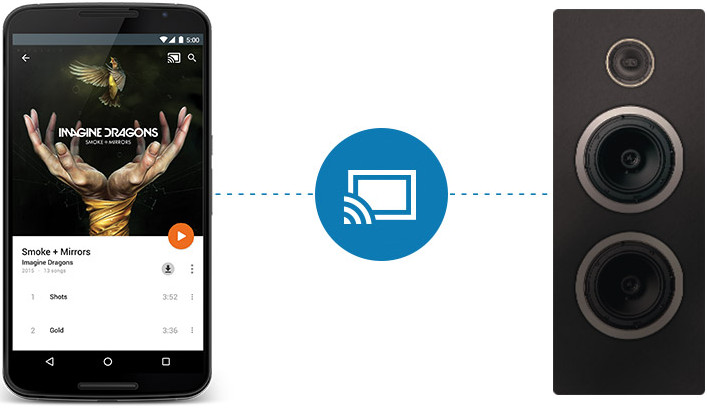
\includegraphics[width=0.65\textwidth]{./Imagenes/cast-speaker.jpg}
	\end{figure}
\end{frame}


\begin{frame}
	\begin{block}{Segundo modo}
		Diseñado para enviar contenido del emisor, como cuando hacemos mirroring o usamos la televisión como segunda pantalla.

		La calidad del streaming en este caso varía según la potencia de procesamiento del emisor. En el caso de un smartphone la calidad
		de las imágenes normalmente se deteriora debido al escalado.
	\end{block}

	\begin{figure}[h]
		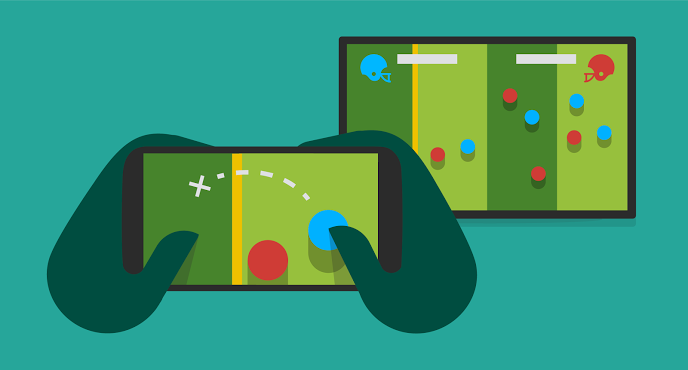
\includegraphics[scale=0.3]{./Imagenes/seconddisplay.png}
	\end{figure}
\end{frame}


\begin{frame}{Comparativa}
	\begin{minipage}[b]{.45\textwidth}
		\centering
		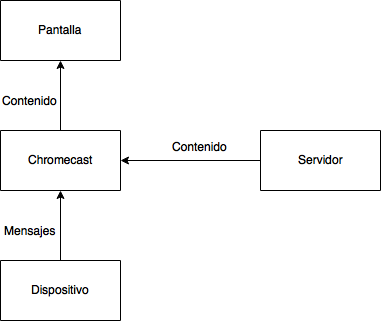
\includegraphics[scale=0.52]{./Imagenes/ChromecastModo1.png}
		%\caption{Primer modo}
	\end{minipage}\qquad
	\hspace{1.65cm}
	\begin{minipage}[b]{.3\textwidth}
		\centering
		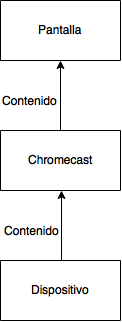
\includegraphics[scale=0.52]{./Imagenes/ChromecastModo2.png}
		%\caption{Segundo modo}
	\end{minipage}
\end{frame}
